\documentclass[a4paper,11pt]{article}

\usepackage[utf8x]{inputenc}
\usepackage[T1]{fontenc}
\usepackage[francais]{babel}
\usepackage{amsmath,amssymb}
\usepackage{fullpage}
\usepackage{xspace}
\usepackage{verbatim}
\usepackage{graphicx}
\usepackage{listings}
\usepackage[usenames,dvipsnames]{color}
\usepackage{url}

\lstset{basicstyle=\small\tt,
  keywordstyle=\bfseries\color{Orchid},
  stringstyle=\it\color{Tan},
  commentstyle=\it\color{LimeGreen},
  showstringspaces=false}

\newtheorem{exo}{Exercice}

\newcommand{\dx}{\,dx}
\newcommand{\ito}{,\dotsc,}
\newcommand{\R}{\mathbb{R}}
\newcommand{\C}{\mathbb{C}}
\newcommand{\N}{\mathbb{N}}
\newcommand{\Poly}[1]{\mathcal{P}_{#1}}
\newcommand{\abs}[1]{\left\lvert#1\right\rvert}
\newcommand{\norm}[1]{\left\lVert#1\right\rVert}
\newcommand{\pars}[1]{\left(#1\right)}
\newcommand{\bigpars}[1]{\bigl(#1\bigr)}
\newcommand{\set}[1]{\left\{#1\right\}}

\title{Compte rendu TP Scilab}
\author{Michel Yoeung}
\date{22 Novembre 2017}

% ===============
\begin{document}
% ===============
\maketitle

%======================================
\section{Sensibilisation à l'arithmétique machine}
%======================================

\begin{exo} \ \\ \\
On obtient $ z=0 $ et $ w=1 $. \\
Pour z, on évalue en premier $ y+x $ : $ 1e(30)+1e(-8) $ qui vaut toujours $ 1e(30) $ (pour Scilab) car le nombre de chiffres significatifs dépasse la limite de chiffres que peut gérer Scilab. On aura par conséquent, $ 1e(30)-1e(30) $ qui vaut 0 donc $ z=0 $. \\
Pour w, on évalue en premier $ x-x $ qui vaut 0 puis $ \frac{1e(-8)}{1e(-8)} $ qui vaut 1 donc $ w=1 $.
\end{exo}

\begin{exo} \ \\ \\
\begin{figure}[h]
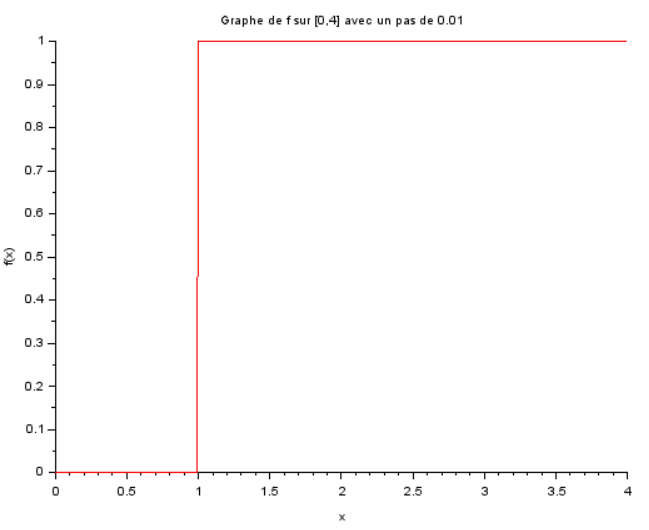
\includegraphics[scale=0.9]{../annexes/courbe_racine.PNG}
\end{figure} \ \\
Lorsque $ x \in [0,1[, f(x)=0 $ car lorsqu'on répète la racine, on va s'approcher de $ 1 $ mais sans jamais être égal à $ 1 $ pile (un moment donné, la valeur de la racine carrée sera bloquée à la valeur juste en dessous de $ 1 $). Donc lorsqu'on va répéter les carrés par la suite, le résultat va décroître jusqu'à atteindre $ 0 $. \ \\
Lorsque $ x=1 $, enchainer les racines carrées et les carrées ne change rien et $ f(x)=1 $ toujours. \ \\
Lorsque $ x \in ]1,4], f(x)=1 $ car lorsqu'on répète la racine carrée, le résultat va décroître jusqu'à atteindre $ 1 $. Donc, lorsqu'on va répéter les carrés par la suite, le résultat va rester à $ 1 $.

\end{exo}

% =============
\end{document}
% =============
